\documentclass[12pt,a4paper]{article}
\usepackage[utf8]{inputenc}
\usepackage[T1]{fontenc}
\usepackage{amsmath}
\usepackage{amsfonts}
\usepackage{amssymb}
\usepackage{graphicx}
\usepackage[indonesian]{babel}
\usepackage[left=2.00cm, right=2.00cm, top=2.00cm, bottom=2.00cm]{geometry}
\usepackage{float} 

\title{Tugas 11 - Pengolahan Sinyal Digital\\
	Representasi dari Linear Digital Networks}

% remove spacing around date:
\usepackage{titling}
\predate{}
\postdate{}
\date{}

\begin{document}
	\maketitle
	\date{}
	\begin{enumerate}
		\item Diketahui sistem waktu diskrit yang direpresentasikan oleh persamaan linear constant-coefficient difference \[ y(n) - \frac{3}{4} y(n-1) + \frac{1}{8} y(n-2) = x(n) \]
		\begin{enumerate}
			\item Gambarkan representasi diagram blok dari sistem dalam bentuk adder dan delay dan coefficient multiplication branch.\\
			\textbf{Jawaban:}\\
			
			\begin{figure}[H]
				\centering
				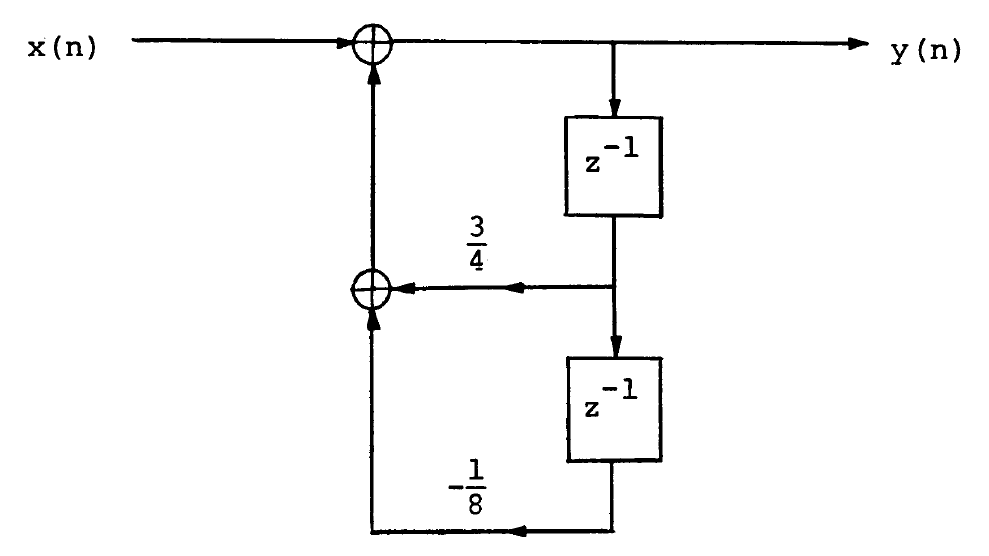
\includegraphics[width=0.5\linewidth]{img/img01}
				\caption{diagram blok sistem}
				\label{fig:img01}
			\end{figure}
			
			\item Gambarkan representasi linear signal-flow dari sistem.\\
			\textbf{Jawaban:}\\
			\begin{figure}[H]
				\centering
				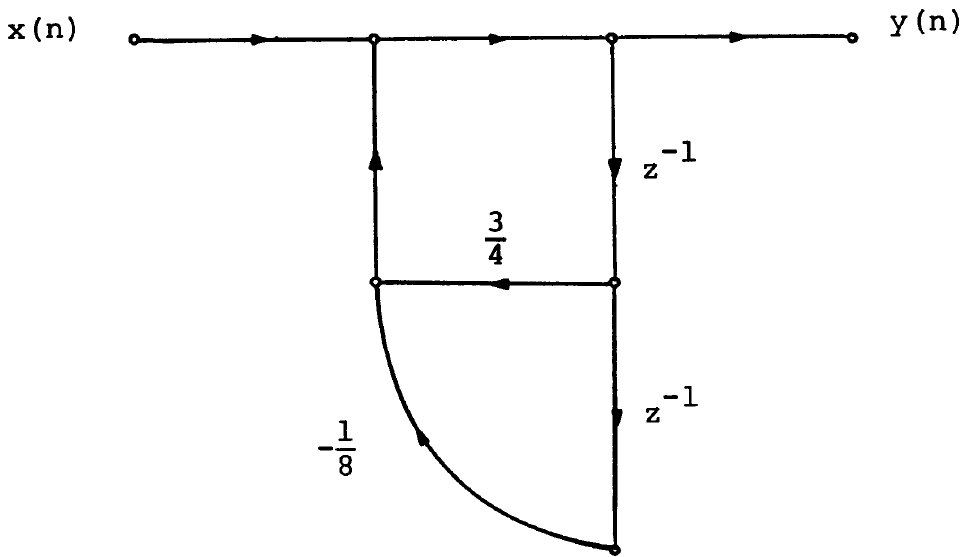
\includegraphics[width=0.5\linewidth]{img/img02}
				\caption{linear signal-flow sistem}
				\label{fig:img02}
			\end{figure}
			
			atau
			
			\begin{figure}[H]
				\centering
				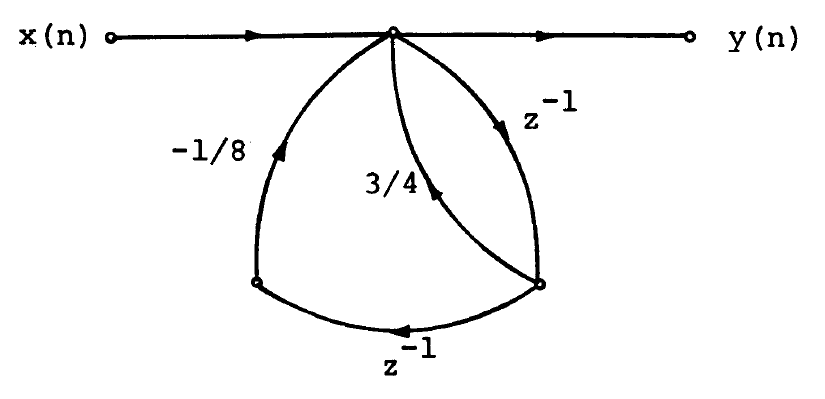
\includegraphics[width=0.5\linewidth]{img/img03}
				\caption{linear signal-flow sistem}
				\label{fig:img03}
			\end{figure}
			
		\end{enumerate}
		\item Diketahui jaringan digital yang ditunjukkan oleh Gambar \ref{fig:img04}
		
		\begin{figure}[H]
			\centering
			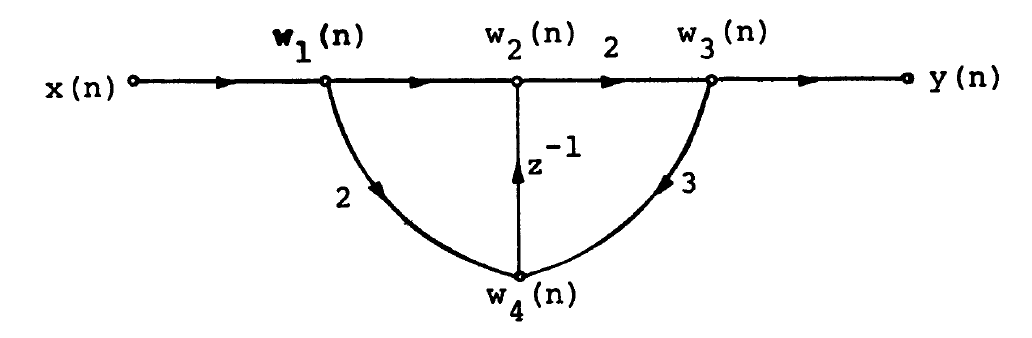
\includegraphics[width=0.5\linewidth]{img/img04}
			\caption{jaringan digital}
			\label{fig:img04}
		\end{figure}
		
		\begin{enumerate}
			\item Untuk jaringan ini, tentukan matriks $ F^t $, $ B^t $, dan $ C^t $.
			\item Tentukan matriks $ F_c^t $ dan $ F_d^t $ di representasi matriks bentuk alternatif.\\
		\end{enumerate}
		\textbf{Jawaban:}
		
		\begin{figure}[H]
			\centering
			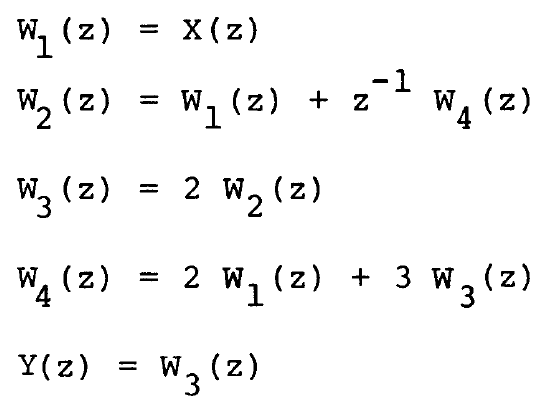
\includegraphics[width=0.3\linewidth]{img/img05}
		\end{figure}
		
		\begin{figure}[H]
			\centering
			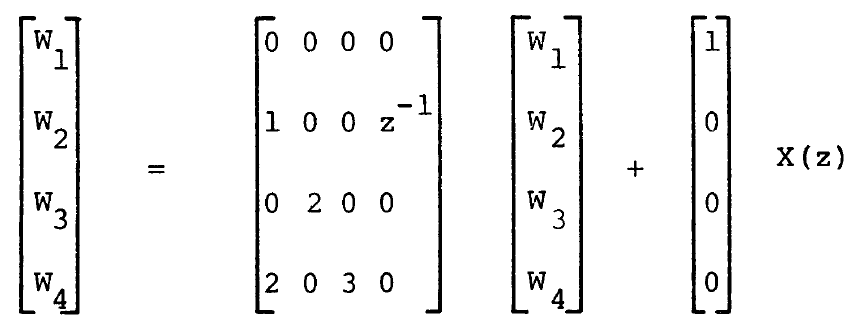
\includegraphics[width=0.5\linewidth]{img/img06}
		\end{figure}
		
		\begin{figure}[H]
			\centering
			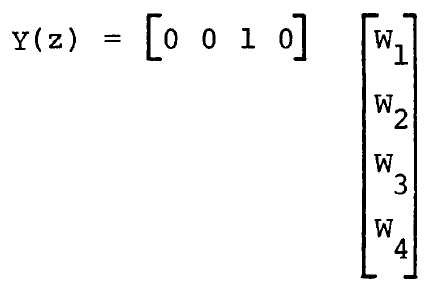
\includegraphics[width=0.3\linewidth]{img/img07}
		\end{figure}
		
		\begin{figure}[H]
			\centering
			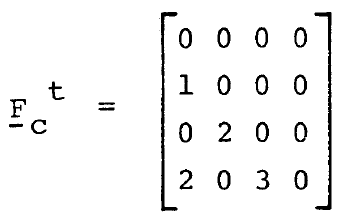
\includegraphics[width=0.2\linewidth]{img/img08}
		\end{figure}
	
		\begin{figure}[H]
			\centering
			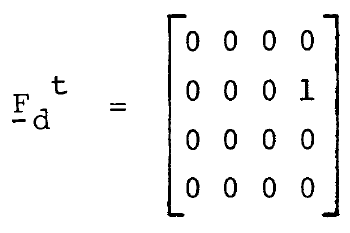
\includegraphics[width=0.2\linewidth]{img/img09}
		\end{figure}
	\end{enumerate}
\end{document}